\section{Бинаризация признаков}

Бинаризация признаков – это процесс преобразования исходных признаков в бинарные переменные, которые принимают значения \(0\) или \(1\). 
%Этот метод широко используется в задачах %машинного обучения, особенно в логических %методах классификации, где входные данные %должны быть представлены в виде набора %булевых предикатов.

\subsection{Бинаризация количественных признаков}

Для признака \( f: X \to D_f \), где \( D_f \) – множество возможных значений признака, бинаризация заключается в создании предикатов, проверяющих выполнение определённых условий. Эти предикаты позволяют разбить множество значений признака на подмножества, которые можно использовать в логических моделях.

В зависимости от типа признака, бинаризация осуществляется следующим образом:
\begin{itemize}
    \item \textbf{Номинальный признак} (\(f\) принимает конечное множество значений, без упорядоченности):
    \[
    \beta(x) = [f(x) = d], \quad d \in D_f;
    \]
    \[
    \beta(x) = [f(x) \in D'], \quad D' \subset D_f.
    \]
    \item \textbf{Порядковый или количественный признак} (\(f\) принимает значения, между которыми можно определить порядок):
    \[
    \beta(x) = [f(x) \leq d], \quad d \in D_f;
    \]
    \[
    \beta(x) = [d \leq f(x) \leq d'], \quad d, d' \in D_f, \, d < d'.
    \]
\end{itemize}

Для количественных признаков (\(f: X \to \mathbb{R}\)) важно выбирать такие пороговые значения \(d\), которые разделяют выборку на значимые группы. Например, 
%пороги \(d\) могут быть определены как средние значения между %соседними элементами вариационного ряда \(f(x_1), \dots, %f(x_\ell)\), упорядоченного по возрастанию:
\[
d_i = \frac{f^{(i)} + f^{(i+1)}}{2}, \quad f^{(i)} \neq f^{(i+1)}, \; i = 1, \dots, \ell - 1,
\]
где \(f^{(1)} \leq f^{(2)} \leq \dots \leq f^{(\ell)}\) – упорядоченные значения признака. (См. рис)

Такими способами можно получить много разных предикатов. Мы хотим выбрать из них самые ''лучшие'' (в каком-либо смысле). Для этого разобьем диапазон значений признака на зоны.

\begin{figure}
    \centering
    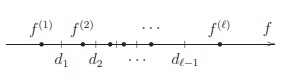
\includegraphics[scale = 1]{chapters/logical/images/bin1.png}
    \caption{Вариационный ряд значений признака $f(x)$ и пороги $d_i$}
\end{figure}

\subsection{Разбиение диапазона значений признака на зоны}

Каждая зона определяется бинарным предикатом:
\begin{align*}
\zeta_0(x) &= [f(x) < d_1], \\
\zeta_s(x) &= [d_s \leq f(x) < d_{s+1}], \quad s = 1, \dots, r-1, \\
\zeta_r(x) &= [d_r \leq f(x)].
\end{align*}

Способы разбиения:
\begin{itemize}
    \item Жадная максимизация информативности путем слияний
    \item Разбиение на равномощные подвыборки
    \item Разбиение по равномерной сетке ''удобных'' значений (например, с минимальным числом значащих цифр)
    \item Объединение нескольких разбиений
\end{itemize}

\subsection{Жадный алгоритм слияния зон}

Алгоритм начинает с разбиения на ''мелкие'' зоны. Пороги проходят между всеми соседними парами точек, принадлежащих \emph{разным} классам, т.~к. расстановка порогов между точками одного класса приведет только к уменьшению информативности зон. Далее зоны укрупняются путём слияния \emph{троек} соседних зон. Зоны сливаются до тех пор, пока
информативность некоторой слитой зоны превышает информативность
исходных зон, либо пока не будет получено заданное количество зон $r$. Каждый раз сливается тройка, дающая наибольший выигрыш в информативности.

\begin{figure}
    \centering
    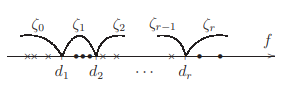
\includegraphics[scale = 1]{chapters/logical/images/bin2.png}
    \caption{Начальное разбиение на зоны}
\end{figure}

\newpage
\textbf{Вход:}
\begin{itemize}
    \item $f(x)$ — признак;
    \item $c \in Y$ — выделенный класс;
    \item $X^\ell = \{(x_i, y_i)\}_{i=1}^\ell$ — выборка, упорядоченная по возрастанию $f(x_i)$;
    \item $r$ — желаемое количество зон;
    \item $\delta_0$ — порог слияния зон (по умолчанию $\delta_0 = 0$).
\end{itemize}

\textbf{Выход:}
\[
D = \{d_1, \dots, d_n\} \text{ — строго возрастающая последовательность порогов;}
\]

\hrule

\begin{enumerate}
    \item $D := \emptyset;$
    \item \textbf{для всех} $i = 2, \dots, \ell$:
    \begin{itemize}
        \item \textbf{если} $f(x_{i-1}) \neq f(x_i)$ и $[y_{i-1} = c] \neq [y_i = c]$ \textbf{то}
        \begin{itemize}
            \item добавить новый порог $d := \frac{f(x_{i-1}) + f(x_i)}{2}$ в конец последовательности $D$;
        \end{itemize}
    \end{itemize}
    \item \textbf{повторять}
    \begin{enumerate}
        \item \textbf{для всех} $d_i \in D, i = 1, \dots, |D| - 1$:
        \begin{itemize}
            \item вычислить выигрыш от слияния тройки соседних зон $\zeta_{i-1}, \zeta_i, \zeta_{i+1}$:
            \[
            \delta_i := I_c(\zeta_{i-1} \cup \zeta_i \cup \zeta_{i+1}) - \max\{I_c(\zeta_{i-1}), I_c(\zeta_i), I_c(\zeta_{i+1})\};
            \]
        \end{itemize}
        \item найти тройку зон, для которой слияние наиболее выгодно:
        \[
        i := \arg \max \delta_i;
        \]
        \item \textbf{если} $\delta_i > \delta_0$ \textbf{то}
        \begin{itemize}
            \item слить зоны $\zeta_{i-1}, \zeta_i, \zeta_{i+1}$, удалить пороги $d_i$ и $d_{i+1}$ из последовательности $D$;
        \end{itemize}
    \end{enumerate}
    \item \textbf{пока} $|D| > r + 1$.
\end{enumerate}

\subsection{Задачи}

\textbf{Задача 1}
Предположим, вы владелец интернет-магазина, и у вас есть данные о стоимости товаров и их популярности (популярен — \( 1 \), непопулярен — \( 0 \)). 
Для анализа спроса вы хотите разбить товары на ценовые зоны, чтобы лучше понять поведение покупателей.

Данные представлены в таблице:

\[
\begin{array}{|c|c|c|}
\hline
\text{№ товара} & \text{Цена товара (\$)} & \text{Популярность } y \\
\hline
1 & 10 & 1 \\
2 & 12 & 1 \\
3 & 15 & 0 \\
4 & 17 & 1 \\
5 & 20 & 0 \\
6 & 23 & 0 \\
7 & 25 & 1 \\
\hline
\end{array}
\]

Как алгоритм слияния зон первично разобьёт выборку на ценовые зоны?

\textbf{Решение}
Рассчитаем пороги:

\[
\begin{aligned}
&d_1 = \frac{12 + 15}{2} = 13.5, \\
&d_2 = \frac{15 + 17}{2} = 16.0, \\
&d_3 = \frac{17 + 20}{2} = 18.5, \\
&d_4 = \frac{23 + 25}{2} = 24.0
\end{aligned}
\]

На основе рассчитанных порогов получаем зоны:

\[
\begin{aligned}
&\zeta_0(x) = [\text{Цена} < 13.5], \\
&\zeta_1(x) = [13.5 \leq \text{Цена} < 16.0], \\
&\zeta_2(x) = [16.0 \leq \text{Цена} < 18.5], \\
&\zeta_4(x) = [29.0 \leq \text{Цена} < 24.0], \\
&\zeta_5(x) = [\text{Цена} \geq 24.0].
\end{aligned}
\]

\textbf{Задача 2}
Будут ли разбиения диапазона меняться в зависимости от класса, относительно которого они производятся? Как изменить алгоритм для получения ''универсального'' разбиения, учитывающего сразу все классы? 

\textbf{Решение}
Да, будут, т.~к. информативность зависит от класса. Нужно заменить критерий информативности многоклассовым критерием.

\textbf{Задача 3}
Какую сложность имеет алгоритм слияния зон? Как можно его ускорить?

\textbf{Решение}
Этот алгоритм имеет трудоёмкость $O(l^2)$. Его можно заметно ускорить, если на каждой итерации сливать не одну тройку зон, а $\tau l$ троек с достаточно большим выигрышем $\delta I_i$, при условии, что они не перекрываются. В этом случае трудоёмкость составляет $O(l / \sqrt{\tau})$.

\section{Взвешенное голосование правил}

Допустим, имеется консилиум экспертов, каждый член которого может допустить ошибку. Процедура голосования — это способ повышения качества принимаемых решений, при котором ошибки отдельных экспертов компенсируют друг друга.

Ранее принцип голосования применялся для построения композиций из произвольных алгоритмов классификации. Теперь рассмотрим композиции, состоящие из логических закономерностей.

\subsection{Принцип голосования}

Пусть для каждого класса $c \in Y$ построено множество логических закономерностей (правил), специализирующихся на различении объектов данного класса:

\[
R_c = \{ \varphi_{tc} : X \to \{0, 1\} \mid t = 1, \dots, T_c \}
\]

Считается, что если $\varphi_{tc}(x) = 1$, то правило $\varphi_{tc}$ относит объект $x \in X$ к классу $c$. Если же $\varphi_{tc}(x) = 0$, то правило воздерживается от классификации объекта $x$.

Алгоритм простого голосования (simple voting) подсчитывает долю правил в наборах $R_c$, относящих объект $x$ к каждому из классов:

\[
\Gamma_c(x) = \frac{1}{T_c} \sum_{t=1}^{T_c} \varphi_{tc}(x), \quad c \in Y,
\]

и относит объект $x$ к тому классу, за который подана наибольшая доля голосов:

\[
a(x) = \arg \max_{c \in Y} \Gamma_c(x).
\]

Если максимум достигается одновременно на нескольких классах, выбирается тот, для которого цена ошибки меньше.

Нормирующий множитель $\frac{1}{T_c}$ вводится для того, чтобы наборы с большим числом правил не перетягивали объекты в свой класс.

\subsection{Алгоритм взвешенного голосования}
Алгоритм взвешенного голосования (weighted voting, WV) действует более тонко, учитывая, что правила могут иметь различную ценность. Каждому правилу $\varphi_{tc}$ приписывается вес $\alpha_{tc} \geq 0$, и при голосовании берется взвешенная сумма голосов:

\[
\Gamma_c(x) = \sum_{t=1}^{T_c} \alpha_{tc} \varphi_{tc}(x), \quad \alpha_{tc} > 0.
\]

Веса нормируются на единицу:

\[
\sum_{t=1}^{T_c} \alpha_{tc} = 1, \quad \forall c \in Y.
\]

Поэтому функцию $\Gamma_c(x)$ называют также выпуклой комбинацией правил $\varphi_1, \dots, \varphi_{T_c}$. Очевидно, простое голосование является частным случаем взвешенного, когда веса одинаковы и равны $\frac{1}{T_c}$.

На первый взгляд, вес правила должен определяться его информативностью. Однако, важно также учитывать, насколько данное правило уникально. Если имеется 10 хороших, но одинаковых (или почти одинаковых) правил, их суммарный вес должен быть сравним с весом столь же хорошего правила, не похожего на все остальные. Таким образом, веса должны учитывать не только ценность правил, но и их различность.

Простой общий подход к настройке весов заключается в том, чтобы сначала найти набор правил $\{ \varphi_{tc}(x) \}$, затем принять их за новые (бинарные) признаки и построить в этом новом признаковом пространстве линейную разделяющую поверхность (кусочно-линейную, если $|Y| > 2$). Для этого можно использовать логистическую регрессию, однослойный персептрон или метод опорных векторов. Существуют и другие подходы. Например, в разделе 1.5.4 будет рассмотрен метод бустинга, в котором правила настраиваются последовательно, и для каждого правила сразу вычисляется его вес.

\subsection{Проблема диверсификации правил}
Голосующие правила должны быть существенно различны, иначе они будут бесполезны для классификации. Продолжая аналогию с консилиумом, заметим, что нет никакого смысла держать в консилиуме эксперта A, если он регулярно подсматривает решения у эксперта B.

Приведем простое теоретико-вероятностное обоснование принципа диверсификации, или повышения различности (diversity) правил \cite{14}. Пусть $X$ — вероятностное пространство, множество ответов $Y$ конечно. Введем случайную величину $M(x)$, равную перевесу голосов в пользу правильного класса; её называют также отступом (margin) объекта $x$ от границы классов:

\[
M(x) = \Gamma_c(x) - \Gamma_{\overline{c}}(x), \quad \Gamma_{\overline{c}}(x) = \max_{y \in Y \setminus \{c\}} \Gamma_y(x), \quad c = y^*(x).
\]

Если отступ положителен ($M(x) > 0$), то алгоритм голосования правильно классифицирует объект $x$. Предположим, что в среднем наш алгоритм классифицирует хотя бы немного лучше, чем наугад: $E[M] > 0$. Тогда можно оценить вероятность ошибки по неравенству Чебышева:

\[
P\{M < 0\} \leq P\{|E[M] - M| > E[M]\} \leq \frac{D_M}{(E[M])^2}.
\]

Отсюда вывод: для уменьшения вероятности ошибки необходимо максимизировать ожидание перевеса голосов $E[M]$ и минимизировать его дисперсию $D_M$. Для выполнения этих условий каждый объект должен выделяться примерно одинаковым числом правил. Обычно ни одно из правил не выделяет класс целиком, поэтому правила должны быть существенно различны, то есть выделять существенно различные подмножества объектов.

Неплохая эвристика, усиливающая различия между правилами и позволяющая равномернее выделять объекты обучения, используется в алгоритме CORAL \cite{12}. Сначала для фиксированного класса $c \in Y$ строится покрывающий набор правил точно так, как это делалось для решающих списков. Затем строится второй покрывающий набор, но при этом запрещается использовать признаки, часто входившие в закономерности первого набора. Поэтому второй набор неминуемо окажется отличным от первого. Затем запрещаются признаки, часто входившие в оба набора, и строится третий набор. И так далее, для каждого класса $c \in Y$.

\subsection{Отказы от классификации}
Возможны ситуации, когда ни одно из правил не выделяет классифицируемый объект $x$. Тогда алгоритм должен либо отказываться от классификации, либо относить объект к классу, имеющему наименьшую цену ошибки. Отказ алгоритма означает, что данный объект является нетипичным, не подпадающим ни под одну из ранее обнаруженных закономерностей. Вообще, обнаружение нетипичности (novelty detection) принято считать отдельным видом задач обучения по прецедентам, наряду с классификацией и кластеризацией. Способность алгоритмов отказываться от классификации нетипичных объектов во многих приложениях является скорее преимуществом, чем недостатком. В то же время, число отказов не должно быть слишком большим.

Итак, при построении алгоритмов взвешенного голосования правил возникает четыре основных вопроса:
\begin{itemize}
    \item Как построить много правил по одной и той же выборке?
    \item Как избежать повторов и построения почти одинаковых правил?
    \item Как избежать появления непокрытых объектов и обеспечить равномерное покрытие всей выборки правилами?
    \item Как определять веса правил при взвешенном голосовании?
\end{itemize}

Рассмотрим, как эти проблемы решаются в известных алгоритмах в следующих параграфах.

\subsection{Задачи}

\textbf{Задача 1: Алгоритм простого голосования}

Допустим, для класса $c \in Y$ существуют 10 правил, которые используют данные для классификации. Каждое правило возвращает 1 или 0 для объекта $x$. Если для объекта $x$ правила 3 и 7 верно классифицируют объект как класс $c$, а остальные возвращают 0, как будет рассчитана доля голосов для класса $c$?

\textbf{Решение:}  
Для класса $c$ доля голосов рассчитывается как сумма всех правил, которые классифицируют объект как класс $c$, делённая на общее количество правил. Если 10 правил, то:
\[
\Gamma_c(x) = \frac{1}{10} \left( 1 + 0 + 0 + 0 + 0 + 0 + 1 + 0 + 0 + 0 \right) = \frac{2}{10} = 0.2
\]
Таким образом, для объекта $x$ доля голосов для класса $c$ составит 0.2.

\textbf{Задача 2: Проблема с весами в алгоритме взвешенного голосования}

В алгоритме взвешенного голосования веса для каждого правила нормируются на единицу. Если для класса $c$ у нас есть 3 правила с весами $\alpha_1 = 0.5$, $\alpha_2 = 0.3$, и $\alpha_3 = 0.2$, как будет выглядеть итоговая сумма голосов $\Gamma_c(x)$, если объект $x$ классифицируется всеми тремя правилами как класс $c$?

\textbf{Решение:}  
Итоговая сумма голосов для класса $c$ рассчитывается по формуле:
\[
\Gamma_c(x) = \sum_{t=1}^{T_c} \alpha_{tc} \varphi_{tc}(x)
\]
где $\varphi_{tc}(x) = 1$, если правило классифицирует объект как класс $c$, и 0 в противном случае. Если все 3 правила классифицируют объект как $c$, то:
\[
\Gamma_c(x) = 0.5 + 0.3 + 0.2 = 1.0
\]

\textbf{Задача 3: Проблема диверсификации правил}

Какова вероятность ошибки при использовании алгоритма голосования, если все правила сильно похожи друг на друга (например, классифицируют одинаковые подмножества объектов)?

\textbf{Решение:}  
Если правила сильно похожи, то вероятность ошибки возрастает. В таких случаях, возможно, правило не будет существенно различать объекты, и алгоритм может ошибаться при классификации новых объектов. Чтобы уменьшить вероятность ошибки, правила должны быть разнообразными, то есть они должны выделять разные подмножества объектов. Для максимизации различий между правилами можно использовать метод, как в алгоритме CORAL, который строит покрывающие наборы правил, постепенно исключая часто встречающиеся признаки.

\textbf{Задача 4: Принцип диверсификации правил}

Пусть для объекта $x$ имеется 10 правил, из которых 8 классифицируют объект как класс $c$, а остальные 2 — как класс $d$. Какой отступ $M(x)$ будет при расчете вероятности правильной классификации?

\textbf{Решение:}  
Отступ для объекта $x$ определяется как разница между голосами для правильного класса и максимальным голосом для всех остальных классов:
\[
M(x) = \Gamma_c(x) - \Gamma_{\overline{c}}(x)
\]
Если из 10 правил 8 голосуют за класс $c$ (доля голосов $0.8$) и 2 — за класс $d$ (доля голосов $0.2$), то:
\[
M(x) = 0.8 - 0.2 = 0.6
\]
Если отступ положителен ($M(x) > 0$), то классификация будет правильной.

\textbf{Задача 5: Отказы от классификации}

Если для объекта $x$ не существует правила, которое его классифицирует, что должен делать алгоритм голосования? Как можно обработать такой случай?

\textbf{Решение:}  
В таком случае алгоритм может либо отказаться от классификации, либо отнести объект к классу с наименьшей ценой ошибки. Такой отказ от классификации часто называют обнаружением нетипичности (novelty detection), что является отдельной задачей в машинном обучении. Важно, чтобы количество отказов не было слишком большим, так как это может снизить эффективность алгоритма.

\section{Алгоритм КОРА}

Алгоритм комбинаторного распознавания КОРА, предложенный М.М.~Бонгардом в 1961 году и реализованный М.Н.~Вайнцвайгом, предназначен для построения набора конъюнктивных закономерностей. Этот алгоритм неоднократно демонстрировал высокую эффективность при решении различных прикладных задач, связанных с распознаванием образов и классификацией.

\subsection{Основные эвристические предположения}

Для эффективной работы алгоритма КОРА сделаны следующие эвристические предположения:

\begin{itemize}
    \item \textbf{Адекватность множества предикатов:} Множество элементарных предикатов \(B\) выбрано таким образом, что среди конъюнкций ранга 2 или 3 уже содержится достаточное количество информативных закономерностей.
    \item \textbf{Ограничение ранга конъюнкций:} Поскольку ранг конъюнкций ограничен числом 3, для поиска закономерностей возможно применение полного перебора, что упрощает процесс поиска.
    \item \textbf{Непротиворечивость закономерностей:} Наибольший интерес представляют те закономерности, которые являются непротиворечивыми, то есть не содержат противоречий в данных.
\end{itemize}

\subsection{Пример дерева перебора}

На рисунке \ref{fig:kora_tree} показано дерево полного перебора конъюнкций в алгоритме КОРА при \(|B| = 4\). Для краткости конъюнкции обозначены номерами составляющих их предикатов.

\begin{figure}[h]
    \centering
    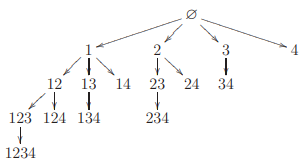
\includegraphics[width=0.6\textwidth]{images/kora_tree.png}
    \caption{Дерево полного перебора конъюнкций в алгоритме КОРА при \(|B| = 4\). Для краткости конъюнкции обозначены номерами составляющих их предикатов.}
    \label{fig:kora_tree}
\end{figure}

\subsection{Описание алгоритма}

Алгоритм КОРА строит конъюнкции, состоящие не более чем из \(K\) термов, выбранных из множества предикатов \(B\). Основой алгоритма является рекурсивная процедура \textit{Нарастить}(\(\varphi\)), которая добавляет термы в конъюнкцию \(\varphi(x)\) всевозможными способами. При этом в список закономерностей \(R_c\) заносятся только наиболее информативные конъюнкции.

\subsubsection{Параметры алгоритма}

Алгоритм использует следующие параметры:

\begin{itemize}
    \item \(D_{\text{min}}\) — минимальная доля позитивных объектов для конъюнкций.
    \item \(E_{\text{max}}\) — максимальная допустимая доля ошибок.
    \item \(T_{\text{min}}, T_{\text{max}}\) — ограничения на количество конъюнкций в списке.
\end{itemize}

\subsubsection{Построение списка информативных конъюнкций методом поиска в глубину (алгоритм КОРА)}

\textbf{Входные данные:}
\begin{itemize}
    \item \(X_\ell\) — обучающая выборка;
    \item \(B\) — семейство элементарных предикатов;
    \item \(K\) — максимальный ранг конъюнкций;
    \item \(E_{\text{max}}\) — максимальная доля ошибок \(E_c(\varphi)\) для конъюнкций \(\varphi \in R_c\);
    \item \(D_{\text{min}}\) — минимальная доля позитивных объектов \(D_c(\varphi)\) для конъюнкций \(\varphi \in R_c\);
    \item \(T_{\text{min}}, T_{\text{max}}\) — ограничения на количество конъюнкций \(T_c\).
\end{itemize}

\textbf{Выходные данные:} 
Списки конъюнкций \(R_c = \{ \varphi_{tc}(x) : t = 1, \dots, T_c \}, \) для всех \(c \in Y\).

\begin{enumerate}
    \item Инициализировать списки: \(R_c = \emptyset\) для всех \(c \in Y\).
    \item Повторять:
    \begin{itemize}
        \item Выполнить \textit{Нарастить}(\(\emptyset\));
        \item Определить \(T := \min_{c \in Y} |R_c|\);
        \item Если \(T < T_{\text{min}}\), то уменьшить \(D_{\text{min}}\) и/или увеличить \(E_{\text{max}}\);
        \item Если \(T > T_{\text{max}}\) или время поиска становится слишком большим, то увеличить \(D_{\text{min}}\) и/или уменьшить \(E_{\text{max}}\);
    \end{itemize}
    \item Пока \(T \notin [T_{\text{min}}, T_{\text{max}})\).
\end{enumerate}

\subsubsection{Процедура \textit{Нарастить}(\(\varphi\))}

\begin{enumerate}
    \item Если \(\varphi = \emptyset\), установить \(j_s := 0\).
    \item Для всех \(j \in \{ j_s + 1, \dots, |B| \}\):
    \begin{itemize}
        \item Добавить терм \(\beta_j\) к исходной конъюнкции:
        \[
        \varphi' := \varphi \wedge \beta_j
        \]
        \item Если \(|\varphi'| \leq K\) и существует \(c \in Y\), такое что:
        \[
        D_c(\varphi') > D_{\text{min}} \quad \text{и} \quad E_c(\varphi') \leq E_{\text{max}},
        \]
        то добавить \(\varphi'\) в список \(R_c\).
        \item Иначе, если \(|\varphi'| < K\) и существует \(c \in Y\), такое что \(D_c(\varphi') > D_{\text{min}}\), то рекурсивно вызвать \textit{Нарастить}(\(\varphi'\)).
    \end{itemize}
\end{enumerate}

\subsubsection{Включение конъюнкции \(\varphi\) в список \(R_c\), содержащий не менее \(T\) самых информативных конъюнкций}

Этот алгоритм предназначен для поддержания в списке \(R_c\) не менее \(T\) самых информативных конъюнкций. Эта процедура обеспечивает управление количеством конъюнкций в списке и поддержание их порядка по информативности.

\begin{enumerate}
    \item \textbf{Процедура} \textit{Добавить\_в\_список}( \(R_c\), \(\varphi\), \(T\) ):
    \item Вставить конъюнкцию \(\varphi\) в список \(R_c\) в порядке убывания информативности \(I_c(\varphi)\).
    \item Найти наименьшую информативность в списке:
    \[
    J := \min_{\psi \in R_c} I_c(\psi)
    \]
    \item Определить количество конъюнкций с наименьшей информативностью:
    \[
    \Delta := \#\{ \psi \in R_c : I_c(\psi) = J \}
    \]
    \item Если \(|R_c| - \Delta > T\), то удалить из списка \(R_c\) все конъюнкции с информативностью \(J\).
\end{enumerate}

\subsection{Достоинства алгоритма КОРА}

\begin{itemize}
    \item \textbf{Интерпретируемость:} Короткие конъюнкции легко интерпретируются в терминах предметной области.
    \item \textbf{Эффективность:} При малых значениях \(K\) (например, \(K \leq 3\)) алгоритм работает очень эффективно.
    \item \textbf{Полнота:} Если существуют короткие информативные конъюнкции, алгоритм обязательно их найдет.
\end{itemize}

\subsection{Недостатки алгоритма КОРА}

\begin{itemize}
    \item \textbf{Зависимость от предикатов:} При неудачном выборе множества предикатов \(B\) короткие информативные конъюнкции могут отсутствовать.
    \item \textbf{Экспоненциальная сложность:} Увеличение числа \(K\) приводит к экспоненциальному росту вычислительной сложности.
    \item \textbf{Отсутствие диверсификации:} Алгоритм не стремится диверсифицировать конъюнкции и обеспечивать равномерное покрытие объектов.
=======
\section{Алгоритм ТЭМП}

Полный перебор всех конъюнкций ранга не более $K$ требует экспоненциального по $K$ числа операций. В реальных задачах объём вычислений становится огромным уже при $K > 3$, и от идеи полного перебора приходится отказаться.

Существует две стандартные стратегии перебора конъюнкций: поиск в глубину (depth-first search) и поиск в ширину (breadth-first search). Первая применяется в алгоритме КОРА, вторая — в алгоритме ТЭМП, предложенным Г. С. Лбовым в 1976 году. Поиск в ширину работает немного быстрее, и в него легче встраивать различные эвристики, сокращающие перебор.

В исходном варианте алгоритм ТЭМП выполнял полный перебор всех конъюнкций ранга не более $K$. Ниже описан слегка модифицированный вариант, позволяющий ограничить перебор и увеличить максимальный ранг конъюнкций $K$.

Алгоритм 1.9 начинает процесс поиска закономерностей с построения конъюнкций ранга 1. Для этого отбираются не более $T_1$ самых информативных предикатов из базового множества $\mathcal{B}$. Затем к каждому из отобранных предикатов добавляется по одному терму из $\mathcal{B}$ всеми возможными способами. Получается не более $T_1|\mathcal{B}|$ конъюнкций ранга 2, из которых снова отбираются $T_1$ самых информативных. И так далее. На каждом шаге процесса делается попытка добавить один терм к каждой из имеющихся конъюнкций. Наращивание конъюнкций прекращается либо при достижении максимального ранга $K$, либо когда ни одну из конъюнкций не удаётся улучшить путём добавления терма.

Лучшие конъюнкции, собранные со всех шагов, заносятся в списки $R_c$. Таким образом, списки $R_c$ могут содержать конъюнкции различного ранга.

Параметр $T_1$ позволяет найти компромисс между качеством и скоростью работы алгоритма. При $T_1 = 1$ алгоритм ТЭМП работает исключительно быстро и строит единственную конъюнкцию, добавляя термы по очереди. Фактически, он совпадает с жадным Алгоритмом 1.2. При увеличении $T_1$ пространство поиска расширяется, алгоритм начинает работать медленнее, но находит больше информативных конъюнкций. На практике выбирают максимальное значение параметра $T_1$, при котором поиск занимает приемлемое время. Однако стратегия поиска всё равно остаётся жадной — термы оптимизируются по-отдельности, и при подборе каждого терма учитываются только предыдущие, но не последующие термы.

Для улучшения конъюнкций к ним применяют эвристические методы «финальной шлифовки» — стабилизацию и редукцию.

В результате стабилизации конъюнкции становятся локально неулучшаемыми. Алгоритм в целом становится более устойчивым — при незначительных изменениях в составе обучающей выборки он чаще находит одни и те же закономерности, а значит, улучшается его способность обобщать эмпирические факты.

В результате стабилизации некоторые конъюнкции могут совпасть, и в списке появятся дубликаты. Их удаление предусмотрено на шаге 13. Если список $R_c$ поддерживается отсортированным по информативности, то удаление дубликатов является недорогой операцией, так как достаточно проверять на совпадение только соседние конъюнкции с одинаковой информативностью.

Если задать $T_1 = \infty$, то алгоритм выполнит полный перебор, как в исходном варианте ТЭМП. «Финальная шлифовка» в этом случае не нужна.

\subsection{Алгоритм 1.9. Построение списка информативных конъюнкций методом поиска в ширину (алгоритм ТЭМП)}


\subsection{Алгоритм 1.9: Построение списка информативных конъюнкций методом поиска в ширину}

\textbf{Вход:}
\begin{itemize}
    \item $X_\ell$ --- обучающая выборка;
    \item $\mathcal{B}$ --- семейство элементарных предикатов;
    \item $c \in Y$ --- класс, для которого строится список конъюнкций;
    \item $K$ --- максимальный ранг конъюнкций;
    \item $T_1$ --- число лучших конъюнкций, отбираемых на каждом шаге;
    \item $T_0$ --- число лучших конъюнкций, отбираемых на последнем шаге, $T_0 \leq T_1$;
    \item $I_{\min}$ --- порог информативности;
    \item $E_{\max}$ --- порог допустимой доли ошибок;
    \item $X_k$ --- контрольная выборка для проведения редукции.
\end{itemize}

\textbf{Выход:} Список конъюнкций $R_c = \{\varphi_t^c(x) : t = 1, \dots, T_c\}$.

\begin{enumerate}
    \item $R_c \gets \emptyset$;
    \item Для всех $\beta \in \mathcal{B}$: \texttt{Добавить\_в\_список($R_c$, $\beta$, $T_1$)};
    \item Для всех $k = 2, \dots, K$:
    \begin{enumerate}
        \item Для всех конъюнкций $\varphi \in R_c$ ранга $(k-1)$:
        \begin{enumerate}
            \item Для всех предикатов $\beta \in \mathcal{B}$, которых ещё нет в конъюнкции $\varphi$:
            \begin{enumerate}
                \item Добавить терм $\beta$ к конъюнкции $\varphi$: $\varphi' = \varphi \land \beta$;
                \item Если $I_c(\varphi') > I_{\min}$, $E_c(\varphi') \leq E_{\max}$ и конъюнкции $\varphi'$ нет в $R_c$, то \texttt{Добавить\_в\_список($R_c$, $\varphi'$, $T_1$)}.
            \end{enumerate}
        \end{enumerate}
    \end{enumerate}
    \item Для всех конъюнкций $\varphi \in R_c$:
    \begin{enumerate}
        \item Стабилизация($\varphi$);
        \item Редукция($\varphi$, $X^k$);
    \end{enumerate}
    \item Удалить из списка $R_c$ дублирующие конъюнкции;
    \item Оставить в списке $R_c$ не более $T_0$ лучших конъюнкций.
\end{enumerate}


\subsection{Достоинства алгоритма ТЭМП}

\begin{itemize}
    \item ТЭМП существенно более эффективен, чем КОРА, особенно при поиске конъюнкций ранга больше 3. Он решает поставленную задачу за $O(KT_1|B|\\ell)$ операций, тогда как КОРА имеет трудоёмкость $O(|B|K\\ell)$.
    \item Параметр $T_1$ позволяет управлять жадностью алгоритма и находить компромисс между качеством конъюнкций и скоростью работы алгоритма.
    \item Благодаря простоте и эффективности алгоритм ТЭМП можно использовать в составе других алгоритмов как генератор конъюнкций, достаточно близких к оптимальным.
\end{itemize}

\subsection{Недостатки алгоритма ТЭМП}

\begin{itemize}
    \item Нет гарантии, что будут найдены самые лучшие конъюнкции, особенно при малых значениях параметра $T_1$.
    \item Алгоритм не стремится увеличивать различность конъюнкций, добиваясь равномерного покрытия объектов выборки. Стабилизация и редукция лишь отчасти компенсируют этот недостаток.
    \item Нет настройки коэффициентов $\\alpha_{tc}$; предполагается простое голосование.

\end{itemize}

\subsection{Задачи}

\textbf{Задача 1}  
Рассмотрим множество элементарных предикатов \( B = \{ \beta_1, \beta_2, \beta_3 \} \) и обучающую выборку \( X_\ell \) с классами \( Y = \{A, B\} \). Предположим, что следующие конъюнкции удовлетворяют условиям \( D_{\text{min}} \) и \( E_{\text{max}} \):

\[
\varphi_1 = \beta_1 \wedge \beta_2, \quad \varphi_2 = \beta_2 \wedge \beta_3, \quad \varphi_3 = \beta_1 \wedge \beta_3
\]

Определите, какие из этих конъюнкций будут добавлены в списки \( R_A \) и \( R_B \) после выполнения процедуры \textit{Нарастить}(\(\emptyset\)).

\textbf{Решение}  
Процедура \textit{Нарастить} начинает с пустой конъюнкции и добавляет термы по одному. Проверяем каждую конъюнкцию на удовлетворение условий \( D_{\text{min}} \) и \( E_{\text{max}} \):

\begin{itemize}
    \item \(\varphi_1 = \beta_1 \wedge \beta_2\): Если для класса \(A\) \(D_A(\varphi_1) > D_{\text{min}}\) и \(E_A(\varphi_1) \leq E_{\text{max}}\), то \(\varphi_1\) добавляется в \( R_A \). Аналогично проверяется для класса \(B\).
    \item \(\varphi_2 = \beta_2 \wedge \beta_3\): Аналогично, добавляется в соответствующие списки классов.
    \item \(\varphi_3 = \beta_1 \wedge \beta_3\): Аналогично, добавляется в соответствующие списки классов.
\end{itemize}

Таким образом, все три конъюнкции будут добавлены в списки \( R_A \) и \( R_B \), если они удовлетворяют заданным условиям.

\textbf{Задача 2}  
Предположим, что при использовании алгоритма КОРА параметр \( K \) увеличен с 3 до 4. Объясните, как это повлияет на эффективность алгоритма и количество генерируемых конъюнкций.

\textbf{Решение}  
Увеличение параметра \( K \) с 3 до 4 расширяет максимальный ранг конъюнкций, позволяя создавать более сложные правила с дополнительным термом. Однако это приводит к экспоненциальному росту числа возможных конъюнкций, что значительно снижает эффективность алгоритма из-за увеличения вычислительной сложности. Кроме того, при большем \( K \) может возрастать вероятность переобучения, так как алгоритм будет генерировать больше конъюнкций, что может привести к снижению обобщающей способности модели.

\textbf{Задача 3}  
Рассмотрим ситуацию, когда множество предикатов \( B \) плохо выбрано, и среди конъюнкций ранга 2 или 3 отсутствуют информативные закономерности. Как это повлияет на работу алгоритма КОРА и какие меры можно предпринять для улучшения результатов?

\textbf{Решение}  
Если множество предикатов \( B \) плохо выбрано и среди конъюнкций ранга 2 или 3 отсутствуют информативные закономерности, алгоритм КОРА не сможет эффективно выявить необходимые закономерности, что приведет к низкой точности классификации. Для улучшения результатов можно предпринять следующие меры:

\begin{enumerate}
    \item \textbf{Пересмотр множества предикатов \( B \):} Добавить новые предикаты или изменить существующие, чтобы повысить их информативность.
    \item \textbf{Увеличение максимального ранга \( K \):} Хотя это снижает эффективность, иногда требуется более высокий ранг для захвата сложных закономерностей.
    \item \textbf{Использование методов отбора признаков:} Применить методы отбора признаков для выбора наиболее информативных предикатов, что может улучшить качество конъюнкций.
    \item \textbf{Комбинирование с другими алгоритмами:} Интегрировать КОРА с другими алгоритмами машинного обучения для улучшения общего качества модели.
\end{enumerate}

Эти меры помогут повысить информативность конъюнкций и, соответственно, эффективность алгоритма КОРА.

\textbf{Задача 1.}
\newline
Рассмотрите граф $G = (V, E)$, где $V = \{A, B, C, D, E\}$ и $E = \{(A, B), (A, C), (B, D), (C, D), (D, E)\}$. Как алгоритм ТЭМП выполняет поиск в ширину для этого графа? Предложите, как можно выполнить поиск в глубину.

\textit{Решение:}
\begin{enumerate}
    \item Алгоритм ТЭМП начинает с вершины $A$, добавляя её соседей $B$ и $C$ в очередь. Затем из очереди выбирается вершина $B$, её сосед $D$ добавляется в очередь, и так далее.
    \item Для поиска в глубину из вершины $A$ алгоритм выбирает один путь (например, $A \to B \to D \to E$), пока не дойдёт до конца, затем возвращается и ищет другие пути.
\end{enumerate}

\textbf{Задача 2.}
\newline
Пусть у нас есть множество предикатов $B = \beta_1, \beta_2, \beta_3$ и максимальный ранг $K = 2$. Какое количество конъюнкций будет проверено алгоритмом ТЭМП, если для каждого шага выбирается $T_1 = 2$? Если мы увеличим $T_1$ до 3, как это повлияет на количество проверяемых конъюнкций?

\textit{Решение:}
\begin{itemize}
    \item При $T_1 = 2$ для ранга 1 будет 2 конъюнкции, для ранга 2 --- $2 \times 3 = 6$ конъюнкций. Всего будет проверено $2 + 6 = 8$ конъюнкций.
    \item Если $T_1 = 3$, то для ранга 1 будет 3 конъюнкции, для ранга 2 --- $3 \times 3 = 9$ конъюнкций. Всего будет проверено $3 + 9 = 12$ конъюнкций.
\end{itemize}

\textbf{Задача 3.}
\newline
Представьте, что вы используете алгоритм ТЭМП для обучения модели с большим количеством предикатов. Какой будет влияние на время вычислений, если вы увеличите $T_1$ с 1 до 5? Объясните это с точки зрения расширения пространства поиска.

\textit{Решение:}
\begin{itemize}
    \item При $T_1 = 1$ алгоритм будет проверять только по одному терму для каждой конъюнкции на каждом шаге, что будет довольно быстрым, но может не давать лучшие результаты.
    \item При увеличении $T_1$ до 5 пространство поиска расширяется, так как на каждом шаге будет добавляться больше термов к конъюнкциям, что увеличивает количество проверяемых комбинаций и тем самым замедляет процесс.
    \item В результате увеличение $T_1$ может существенно замедлить алгоритм, но при этом улучшится качество найденных решений.
\end{itemize}


\section*{Критерии информативности}

Решающие деревья являются одним из базовых методов машинного обучения, который используется как для задач классификации, так и для задач регрессии. Одним из ключевых аспектов построения эффективных деревьев является выбор критериев, определяющих, насколько информативен тот или иной сплит. Эти критерии играют решающую роль в формировании структуры дерева, определяя его глубину, разбиения и качество предсказаний. 

В данной статье мы рассмотрим популярные подходы к определению информативности сплитов в зависимости от постановки задачи. Мы детально разберем критерии, применяемые в задачах регрессии (среднеквадратичная ошибка, средняя абсолютная ошибка) и классификации (энтропия, критерий Джини и другие).


\subsection*{Информативность в задаче регрессии: MSE}
Посмотрим на простой пример - регрессию с минимизацией среднеквадратичной ошибки:

\[
L\left(y_{i}, c\right)=\left(y_{i}-c\right)^{2}
\]

Информативность листа будет выглядеть следующим образом:

\[
H\left(X_{m}\right)=\frac{1}{\left|X_{m}\right|} \min _{c \in Y} \sum_{\left(x_{i}, y_{i}\right) \in X_{m}}\left(y_{i}-c\right)^{2}
\]

Как мы уже знаем, оптимальным предсказанием константного

классификатора для задачи минимизации MSE является среднее значение, то есть
\[
\(c=\frac{\sum y_{i}}{\left|X_{m}\right|}\)
\]

Подставив в формулу информативности сплита, получаем:
\[
H(X_m) = \sum_{(x_i, y_i) \in X_m} \frac{(y_i - \overline{y})^2}{|X_m|}, \quad \text{где } \overline{y} = \frac{1}{|X_m|} \sum_i y_i
\]

То есть при жадной минимизации MSE информативность - это оценка дисперсии таргетов для объектов, попавших в лист. Получается очень стройная картинка: оценка значения в каждом листе - это среднее, а выбирать сплиты надо так, чтобы сумма дисперсий в листьях была как можно меньше.

\subsection*{Информативность в задаче регрессии: MAE}
\[
\(L\left(y_{i}, c\right)=\left|y_{i}-c\right|\)
\]

Случай средней абсолютной ошибки так же прост: в листе надо предсказывать медиану, ведь именно медиана таргетов для обучающих примеров минимизирует MAЕ констатного предсказателя (мы это обсуждали в параграфе про линейные модели).

В качестве информативности выступает абсолютное отклонение от медианы:

\[
H\left(X_{m}\right)=\sum_{\left(x_{i}, y_{i}\right) \in X_{m}} \frac{\left|y_{i}-M E D I A N(Y)\right|}{\left|X_{m}\right|}
\]

\subsection*{Критерий информативности в задаче классификации: misclassification error}
Пусть в нашей задаче \(K\) классов, а \(p_{k}\) - доля объектов класса \(k\) в текущей вершине \(X_{m}\) :
\[
\(p_{k}=\frac{1}{\left|X_{m}\right|} \sum_{\left(x_{i}, y_{i}\right) \in X_{m}} \mathbb{I}\left[y_{i}=k\right]\)
\]

Допустим, мы заботимся о доле верно угаданных классов, то есть функция потерь - это индикатор ошибки:
\[
\(L\left(y_{i}, c\right)=\mathbb{I}\left[y_{i} \neq c\right]\)
\]
Пусть также предсказание модели в листе - один какой-то класс. Информативность для такой функции потерь выглядит так:

\[
H\left(X_{m}\right)=\min _{c \in Y} \frac{1}{\left|X_{m}\right|} \sum_{\left(x_{i}, y_{i}\right) \in X_{m}} \mathbb{I}\left[y_{i} \neq c\right]
\]

Ясно, что оптимальным предсказанием в листе будет наиболее частотный класс \(k_{*}\), а выражение для информативности упростится следующим образом:

\[
H\left(X_{m}\right)=\frac{1}{\left|X_{m}\right|} \sum_{\left(x_{i}, y_{i}\right) \in X_{m}} \mathbb{I}\left[y_{i} \neq k_{*}\right]=1-p_{k_{*}}
\]

\subsection*{Информативность в задаче классификации: энтропия}
Если же мы собрались предсказывать вероятностное распределение классов \(\left(c_{1}, \ldots, c_{K}\right)\), то к этому вопросу можно подойти так же, как мы поступали при выводе логистической регрессии: через максимизацию логарифма правдоподобия (= минимизацию минус логарифма) распределения Бернулли. А именно, пусть в вершине дерева предсказывается фиксированное распределение \(с\) (не зависящее от \(x_{i}\) ), тогда правдоподобие имеет вид

\[
P(y \mid x, c) = P(y \mid c) = \prod_{(x_i, y_i) \in X_m} P(y_i \mid c) = \prod_{(x_i, y_i) \in X_m} \prod_{k=1}^K c_k^{\mathbb{I}[y_i = k]},
\]
откуда
\[
H(X_m) = \min_{\sum_k c_k = 1} \left( - \frac{1}{|X_m|} \sum_{(x_i, y_i) \in X_m} \sum_{k=1}^K \mathbb{I}[y_i = k] \log c_k \right).
\]

То, что оценка вероятностей в листе \(c_{k}\), минимизирующая \(H\left(X_{m}\right)\), должна быть равна \(p_{k}\), то есть доле попавших в лист объектов этого класса, до некоторой степени очевидно, но это можно вывести и строго.

Подставляя вектор \(c=\left(p_{1}, \ldots, p_{K}\right)\) в выражение выше, мы в качестве информативности получим энтропию распределения классов:

\[
H\left(X_{m}\right)=-\sum_{k=1}^{K} p_{k} \log p_{k}
\]

\subsection*{Информативность в задаче классификации: критерий Джини}
Пусть предсказание модели - это распределение вероятностей классов \(\left(c_{1}, \ldots, c_{k}\right)\). Вместо логарифма правдоподобия в качестве критерия можно выбрать, например, метрику Бриера (за которой стоит всего лишь идея посчитать MSE от вероятностей). Тогда информативность получится равной

\[
H\left(X_{m}\right)=\min _{\sum_{k} c_{k}=1} \frac{1}{\left|X_{m}\right|} \sum_{\left(x_{i}, y_{i}\right) \in X_{m}} \sum_{k=1}^{K}\left(c_{k}-\mathbb{I}\left[y_{i}=k\right]\right)^{2}
\]

Можно показать, что оптимальное значение этой метрики, как и в случае энтропии, достигается на векторе \(c\), состоящем из выборочных оценок частот классов \(\left(p_{1}, \ldots, p_{k}\right), p_{i}=\frac{1}{\left|X_{m}\right|} \sum_{i} \mathbb{I}\left[y_{i}=k\right]\). Если подставить
\(\left(p_{1}, \ldots, p_{k}\right)\) в выражение выше и упростить его, получится критерий Джини:
\[
\(H\left(X_{m}\right)=\sum_{k=1}^{K} p_{k}\left(1-p_{k}\right)\)
\]
Критерий Джини допускает и следующую интерпретацию: \(H\left(X_{m}\right)\) равно математическому ожиданию числа неправильно классифицированных объектов в случае, если мы будем приписывать им случайные метки из дискретного распределения, заданного вероятностями \(\left(p_{1}, \ldots, p_{k}\right)\).

\subsection*{Неоптимальность полученных критериев}
Казалось бы, мы вывели критерии информативности для всех популярных задач, и они довольно логично следуют из их постановок, но получилось ли у нас обмануть NP-полноту и научиться строить оптимальные деревья легко и быстро?

Конечно, нет. Простейший пример - решение задачи XOR с помощью жадного алгоритма и любого критерия, который мы построили выше:\\
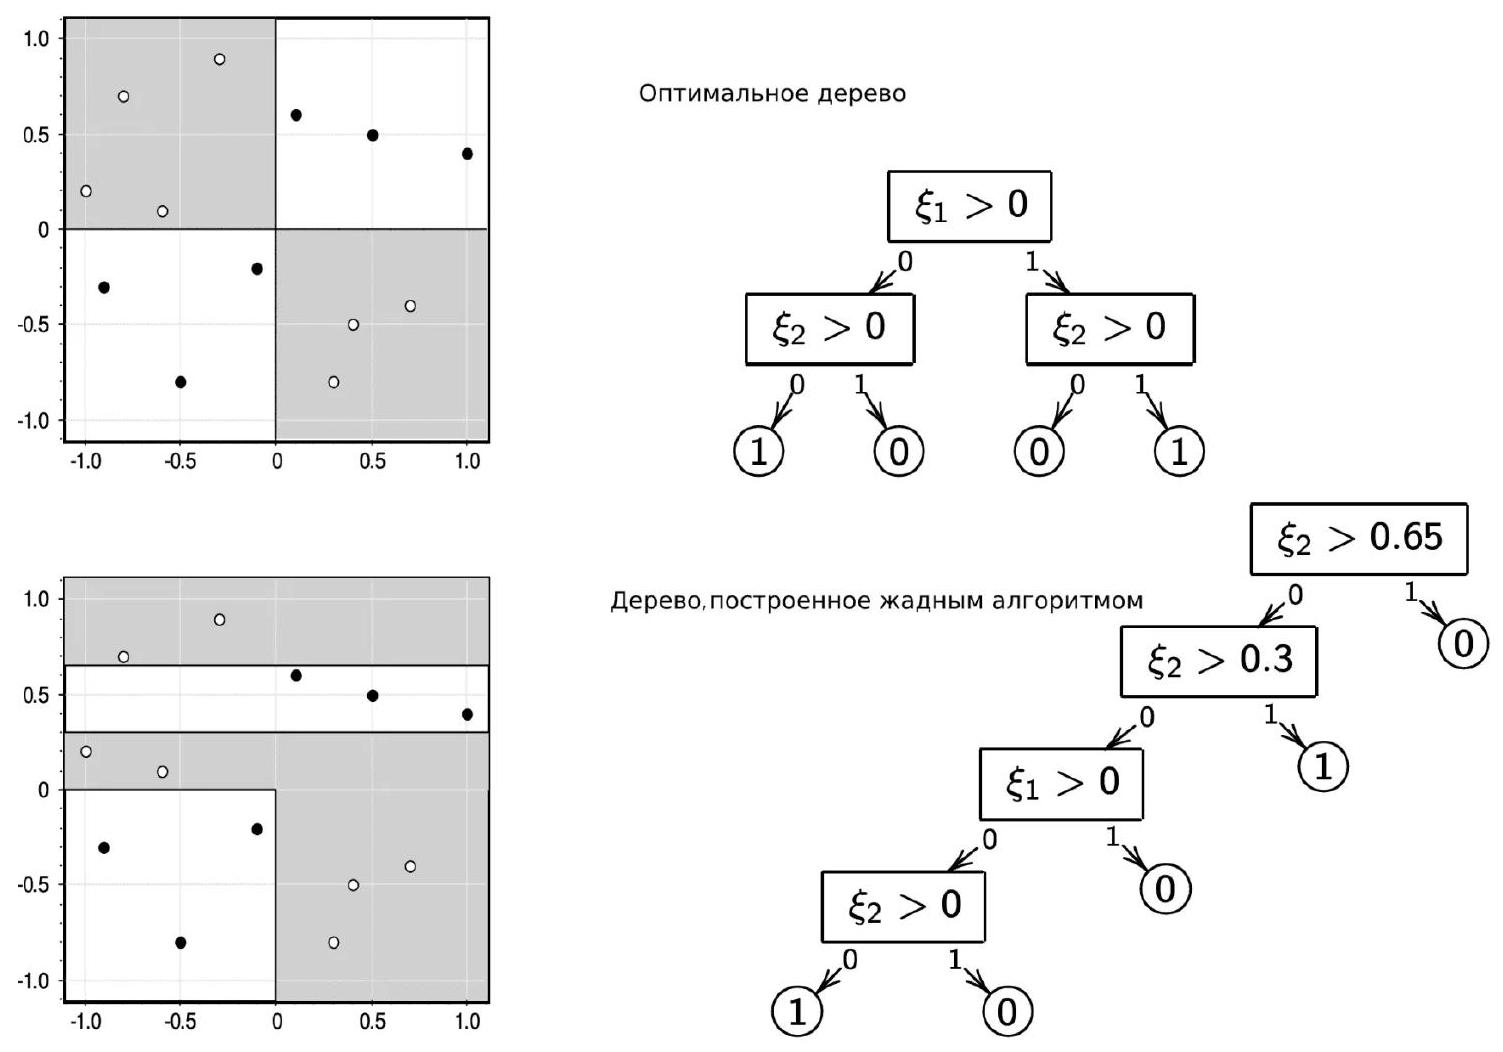
\includegraphics[width=\textwidth, center]{2024_12_13_74602cb5a186ed81f4bcg-8}

Вне зависимости от того, что вы оптимизируете, жадный алгоритм не даст оптимального решения задачи XOR. Но этим примером проблемы не исчерпываются. Скажем, бывают ситуации, когда оптимальное с точки зрения выбранной метрики дерево вы получите с критерием ветвления, построенным по другой метрике (например, MSE-критерий для MAE-задачи или Джини для misclassification error).


\subsection*{Задача 1. Информативность в задаче регрессии (MSE)}

Пусть в лист \(X_m\) попали объекты \(\{(x_i, y_i)\}_{i=1}^n\), и мы рассматриваем критерий информативности для задачи регрессии с квадратичной функцией потерь. Покажите, что минимизация средней квадратичной ошибки в листе приводит к выбору среднего значения таргета \(\overline{y}\) в качестве предсказания, а сама информативность листа равна дисперсии ответов в этом листе. Формально, если

\[
H(X_m) = \frac{1}{n} \sum_{i=1}^n (y_i - c)^2,
\]

то найдите \(c\), минимизирующее \(H(X_m)\), и подставив его обратно, выразите \(H(X_m)\) через \(\overline{y}\) и \(\{y_i\}\).

\subsubsection*{Решение к Задаче 1}

Для функции

\[
H(X_m) = \frac{1}{n} \sum_{i=1}^n (y_i - c)^2
\]

найдём минимум по \(c\). Рассчитаем производную:

\[
\frac{\partial H}{\partial c} = \frac{2}{n} \sum_{i=1}^n (c - y_i).
\]

Приравнивая её к нулю:

\[
\sum_{i=1}^n (c - y_i) = 0 \implies nc - \sum_{i=1}^n y_i = 0 \implies c = \frac{1}{n}\sum_{i=1}^n y_i = \overline{y}.
\]

Таким образом, оптимальное предсказание — среднее значение таргета. Подставляя \(c = \overline{y}\) в \(H(X_m)\), получаем:

\[
H(X_m) = \frac{1}{n} \sum_{i=1}^n (y_i - \overline{y})^2.
\]

Заметим, что это именно выборочная дисперсия (без нормировки на \(n-1\)) таргетов в листе. Таким образом, минимизация MSE соответствует минимизации дисперсии в листьях.


\subsection*{Задача 2. Критерии информативности в задаче классификации}

Пусть в листе \(X_m\) выборки для задачи классификации имеется \(K\) классов, а доля \(k\)-го класса равна \(p_k\). Покажите, что для следующих критериев информативности минимизирующий их вектор вероятностей \(c = (c_1, \ldots, c_K)\) равен \(p = (p_1, \ldots, p_K)\):

1. Ошибка классификации (misclassification error): 
\[
H(X_m) = 1 - \max_k p_k.
\]

2. Энтропия:
\[
H(X_m) = -\sum_{k=1}^K p_k \log p_k.
\]

3. Критерий Джини:
\[
H(X_m) = \sum_{k=1}^K p_k(1 - p_k).
\]

Поясните, почему для всех этих критериев наилучшее предсказание в листе — это вектор оценочных вероятностей классов, равных их эмпирическим частотам.

\subsubsection*{Решение к Задаче 2}

Рассмотрим три критерия информативности.

1. \textbf{Ошибка классификации}: 
Оптимальное предсказание — класс, встречающийся чаще всего, поскольку минимизируется число ошибок. Индикаторная функция ошибки достигает минимума при выборе класса \(k_*\), для которого \(p_{k_*} = \max_k p_k\). Но если мы хотим предсказывать распределение, то его оптимальный вариант — вектор, в котором единица стоит на месте наиболее вероятного класса, что соответствует выборочным частотам (для детерминированного предсказания).

2. \textbf{Энтропия}:
Энтропия минимизируется при вырожденном распределении (когда все массы сосредоточены в одной точке), однако в условиях задачи мы хотим получить оценку, согласованную с данными. В постановке с логарифмом правдоподобия оптимальное распределение классов \((c_1,\ldots,c_K)\) при фиксированных \((y_i)\) достигается при \(c_k = p_k\). Строгий вывод следует из решения задачи оптимизации с ограничением \(\sum_k c_k = 1\). Применение метода Лагранжа приводит к тому, что минимум достигается при совпадении \(c_k\) и \(p_k\).

3. \textbf{Критерий Джини}:
Показатель Джини интерпретируется как ожидаемая ошибка при случайной приписке метки объекта согласно предсказанному распределению. Аналогично энтропии, решение задачи оптимизации даёт \(c_k = p_k\).

Во всех трёх случаях оптимальное распределение в листе совпадает с эмпирическими частотами классов. Это связано с тем, что все рассмотренные критерии имеют минимум в точке эмпирического распределения, отражающего фактические данные.


\subsection*{Задача 3. Жадные алгоритмы и их неоптимальность}

Рассмотрим задачу классификации, где истинное решение требует нетривиальной структуры разделяющей поверхности, например задачу XOR. Покажите, что жадный алгоритм построения дерева, независимо от того, используете ли вы критерий энтропии, Джини или ошибку классификации, не сможет за один или два сплита добиться оптимального разделения. Объясните, почему жадность при выборе сплитов может привести к локально оптимальным, но не глобально оптимальным решениям.

\subsubsection*{Решение к Задаче 3}

Задача XOR устроена так, что данные, принадлежащие разным классам, перемешаны таким образом, что никакой простой линейный или однопараметрический сплит не улучшит ситуацию кардинально, если смотреть на локальный шаг. Жадный алгоритм выбирает признак и порог, максимизирующий улучшение критерия информативности в текущий момент, но не учитывает будущую структуру дерева.

При XOR-классификации каждый простой сплит либо оставляет смешанные классы в листьях, либо не даёт существенного выигрыша по критерию информативности. Чтобы идеально решить XOR, дереву потребуется хотя бы несколько уровней разбиений. Однако жадный выбор первого сплита будет неинформативным с точки зрения глобального решения. Таким образом, критерий информативности, основанный на локальных улучшениях, не гарантирует нахождения глобального оптимума.

Такой пример иллюстрирует фундаментальную проблему: оптимизация критерия информативности по листам не решает NP-полную задачу глобального оптимума структуры дерева. Жадный алгоритм может застревать в локальных оптимумах, не достигая оптимального глобального решения.


\section{Решающее дерево}
Среди множества существующих методов классификации особое место занимают решающие деревья.
Можно выделить несколько преимуществ этих моделей.
\begin{enumerate}
    \item \textbf{Простая реализация}: модель представляет собой структуру, напоминающую дерево с узлами и ветвями.
    \item \textbf{Результаты легко интерпретируемы}: решения принимаются на основе последовательных вопросов о характеристиках объектов.
    \item \textbf{Независимость от структуры данных}: решающее дерево может работать как с числовыми, так и с категориальными признаками без предварительной обработки.

\end{enumerate}
Однако, несмотря на множество преимуществ, решающие деревья имеют и некоторые ограничения. Например, они склонны к переобучению, особенно при наличии большого количества признаков или при недостаточной глубине дерева.
Для преодоления этих недостатков были разработаны различные методы регуляризации и оптимизации, позволяющие улучшить общую производительность модели. А так же решающее деревья послужили базой для построения более сложных алгоритмов, таких как градиентный бустинг на деревьях и случайный лес.

\subsection{Моделирование решающих деревьев}
Условимся обозначать через $\mathbb{X}$ множество объектов, поступающих на вход модели, через $\mathbb{Y}$ множество объектов, в которое модель действует. Начнём с определения.
\begin{definition}
    \textit{Решающим деревом} называется бинарное дерево, в котором
    \begin{enumerate}
        \item каждой внутренней вершине $v$ преписан предикат $B_v: \mathbb{X} \to \{0, 1\}$;
        \item каждой листовой вершине $u$ преписан прогноз $c_u \in \mathbb{Y}$.
    \end{enumerate}
\end{definition}

Давайте немного обсудим определение. Во-первых, понятно как получить для входного объекта ответ: применить к нему предикат и, если он равен 1 (0), пойти в правого (левого) сына текущей вершины, а затем повторять процедуру, пока не дошли до листа. Во-вторых, прогнозы, приписанные листовым вершинам, могут иметь любую природу: будь это числовые константы, векторы вероятностей или даже другие модели. Но всё же обычно, останавливаются на предсказании констант (для классификации - номер класса или всё так же вектор вероятностей принадлежности классам).

\begin{example}
    В задаче классификации клиентов банка на категории "кредитоспособный" и "некредитоспособный" решающее дерево может сначала разделить клиентов по уровню дохода, затем по наличию задолженностей и т.д., чтобы в конечном итоге определить вероятность одобрения кредита для каждого клиента.
\end{example}

\subsection{Обучение решающих деревьев}
Процесс обучения решающего дерева включает в себя последовательное разделение данных на подмножества, основываясь на значениях различных признаков, с целью максимизации чистоты классов в каждом узле дерева. А именно, хочется подбирать предикат для каждого узла так, чтобы разбиние данных, доходящих до него, было наилучшим из возможных. Одним из наиболее распространённых подходов к построению решающих деревьев является использование \textit{жадного алгоритма}. Для простоты условимся работать только с так называемыми \textit{пороговыми предикатами}: $B_{j, t} = x_j \leq t$.

Пусть $X$ — обучающая выборка, а $X_m$ — множество объектов в текущем узле (в начале $X_m = X$). Жадный алгоритм строится следующим образом:

\begin{enumerate}
    \item Создаём вершину $v$.
    \item Если выполнен критерий остановки $Stop(X_m)$, объявляем вершину листом с ответом $Ans(X_m)$.
    \item Иначе выбираем предикат $B_{j,t}$, который максимально улучшает критерий ветвления $Branch(X_m, j, t)$, и делим $X_m$ на $X_{\ell}$ и $X_r$.
    \item Для $X_{\ell}$ и $X_r$ повторяем процесс рекурсивно.
\end{enumerate}

Алгоритм использует вспомогательные функции:
\begin{itemize}
    \item $Ans(X_m)$ — ответ в листе. Например, для классификации это самый частый класс или распределение вероятностей, для регрессии — среднее значение, медиана или простая модель.
    \item $Stop(X_m)$ — правило остановки, срабатывающее, если данные в узле достаточно однородны или их слишком мало.
    \item $Branch(X_m, \textit{feature}, \textit{value})$ — оценка качества разбиения. Выбирается предикат, дающий наибольшее улучшение.
\end{itemize}

Как правило, $Ans(X_m)$ и $Branch(X_m, \textit{feature}, \textit{value})$ подбираются во время обучения дерева, а функция $Stop(X_m)$ выступает гиперпараметром построения этого дерева.
Самым интересным является подборр функции для узла, обеспечивающий наилучшее разбиение. Об этом стоит поговорить подробнее.

\subsection{Критерии ветвления}
Ответы дерева можно представлять в виде $c \in \mathbb{R}$ для задач регрессии и меток классов. В случаях, когда требуется предсказать вероятностное распределение классов, $c$ будет вектором вероятностей, то есть $c \in \mathbb{R}^K$:

\[
c = (c_1, \dots, c_K), \quad \sum_{i=1}^K c_i = 1
\]

Предположим, что задана функция потерь $L(y_i, c)$, которая измеряет качество предсказаний.

При поиске оптимального разбиения $X_m = X_\ell \bigsqcup X_r$ можно вычислить константное значение $c$, которое предсказало бы дерево, если текущая вершина стала бы листом. Это значение выбирается так, чтобы минимизировать среднее значение функции потерь:

\[
\frac{1}{|X_m|} \sum_{(x_i, y_i) \in X_m} L(y_i, c)
\]

Минимальное значение этой функции:

\[
H(X_m) = \min_{c \in Y} \frac{1}{|X_m|} \sum_{(x_i, y_i) \in X_m} L(y_i, c)
\]

называют информативностью или \textit{impurity}. Чем ниже эта величина, тем лучше объекты внутри листа аппроксимируются константным значением.

Критерий ветвления определяется через изменение информативности следующим образом:

\[
Branch(X_m, j, t) = |X_m| \cdot H(X_m) - |X_\ell| \cdot H(X_\ell) - |X_r| \cdot H(X_r)
\]

Интуция здесь следующая: мы смотрим, как хорошо можно приблизить объекты константным значением, если разбить их на две части (естественно константы свои для каждой части), и сравниваем это с информативностью, которую имеем на данный момент.

Получившаяся величина неотрицательна: ведь, разделив объекты на две кучки и подобрав ответ для каждой, мы точно не сделаем хуже. Кроме того, она тем больше, чем лучше предлагаемый сплит.

Остаётся определить функционал качества $L$ и можно обучать дерево. Но для задачи классификации можно определить информативность немного по-другому, что снова заслуживает небольшого отдельного разговора.

\subsection{Энтропия}
Если необходимо предсказывать вероятностное распределение классов $(c_1, \dots, c_K)$, это можно сделать аналогично логистической регрессии. Основной подход заключается в максимизации логарифма правдоподобия (или минимизации его отрицательной величины) для распределения Бернулли. Предположим, что в вершине дерева предсказывается фиксированное распределение $c$, которое не зависит от $x_i$. В этом случае правдоподобие выражается следующим образом:

\[
P(y \mid x, c) = P(y \mid c) = \prod_{(x_i, y_i) \in X_m} P(y_i \mid c) = \prod_{(x_i, y_i) \in X_m} \prod_{k=1}^K c_k^{\mathbb{I}[y_i = k]},
\]

откуда вытекает, что
,
\[
H(X_m) = \min_{\sum_k c_k = 1} \left( -\frac{1}{|X_m|} \sum_{(x_i, y_i) \in X_m} \sum_{k=1}^K \mathbb{I}[y_i = k] \log c_k \right).
\]

\section{Задачи для закрепления материала}
\subsection{Задача 1: Переобучение дерева}
Пусть у вас есть тренировочная выборка из 100 объектов с 10 признаками и тестовая выборка из 30 объектов. Вы построили решающее дерево, которое идеально классифицирует тренировочную выборку (точность 100\%), но на тестовой выборке точность всего 50\%.

\textbf{Вопросы}:
\begin{enumerate}
    \item Почему произошло переобучение?
    \item Какие методы регуляризации можно применить, чтобы уменьшить переобучение?
    \item Как критерий остановки помогает предотвратить переобучение?
\end{enumerate}
\begin{solution}
Причина: дерево слишком сложное (глубокое), оно идеально подстроилось под тренировочные данные, но на тестовых данные из-за слабой обобщающей способности модель показала низкий результат.

Варинты решений:
\begin{enumerate}
    \item Ограничить максимальную глубину (\(\texttt{max\_depth}\)).
    \item Установить минимальное число объектов в листе (\(\texttt{min\_samples\_leaf}\)).
    \item Использовать случайный лес или ансамбли для повышения обобщающей способности.
\end{enumerate}
\end{solution}

\subsection{Задача 2: Вывод энтропийного критерия}
Вернёмся к последнему пункту, а конкретнее к информативности, предложенной в нём:
\[
H(X_m) = \min_{\sum_k c_k = 1} \left( -\frac{1}{|X_m|} \sum_{(x_i, y_i) \in X_m} \sum_{k=1}^K \mathbb{I}[y_i = k] \log c_k \right).
\]
Но причём же тут энтропия? Докажите, что что оценка вероятностей в листе $c_{k}$, минимизирующая $H(X_M)$, должна быть равна $p_k$, то есть доле попавших в лист объектов этого класса. Откуда при подстановке вектора вероятностей $c = (c_1, \dots, c_K)$ получается формула
\[
H(X_m) = - \sum_{k=1}^K p_k \log p_k
\]
\begin{solution}
    Из-за наличия условия $\sum_k c_k = 1$ нам придётся минимизировать лагранжиан:

\[
L(c, \lambda) = \min_{c, \lambda} \left( -\frac{1}{|X_m|} \sum_{(x_i, y_i) \in X_m} \sum_{k=1}^K \mathbb{I}[y_i = k] \log c_k + \lambda \sum_{k=1}^K c_k \right).
\]

Как обычно, возьмём частную производную по $c_j$ и решим уравнение:

\[
0 = \frac{\partial}{\partial c_j} L(c, \lambda) =
\]

\[
= \frac{\partial}{\partial c_j} \left( -\frac{1}{|X_m|} \sum_{(x_i, y_i) \in X_m} \sum_{k=1}^K \mathbb{I}[y_i = k] \log c_k + \lambda \sum_{k=1}^K c_k \right).
\]

Упрощаем производную:

\[
0 = \left( -\frac{1}{|X_m|} \sum_{(x_i, y_i) \in X_m} \mathbb{I}[y_i = j] \frac{1}{c_j} \right) + \lambda.
\]

Решая уравнение относительно $c_j$, получаем:

\[
c_j = \frac{p_j}{\lambda},
\]

где $p_j = \frac{1}{|X_m|} \sum_{(x_i, y_i) \in X_m} \mathbb{I}[y_i = j]$ — доля объектов класса $j$ в текущем узле.

Суммируя эти равенства по $j$, учитывая, что $\sum_k c_k = 1$, находим значение $\lambda$:

\[
1 = \sum_{k=1}^K c_k = \frac{1}{\lambda} \sum_{k=1}^K p_k = \frac{1}{\lambda}.
\]

Таким образом, $\lambda = 1$, и окончательное выражение для $c_j$ имеет вид:

\[
c_j = p_j,
\]

то есть оптимальное значение $c_j$ — это доля объектов класса $j$ в узле $X_m$.
\end{solution}

\subsection{Задача 3: Построение простого дерева}
Дан набор данных:

\[
\begin{array}{|c|c|c|c|}
\hline
\textbf{Объект} & \textbf{Признак 1} & \textbf{Признак 2} & \textbf{Класс} \\
\hline
1 & 5 & 10 & A \\
2 & 6 & 15 & A \\
3 & 7 & 20 & B \\
4 & 8 & 25 & B \\
\hline
\end{array}
\]

Попробуйте построить вручную решающее дерево для классификации этих объектов. Используйте пороговые предикаты вида $B_{j, t} = x_j \leq t$. А в качестве критерия информативности используйте \textit{индекс Джини}

\[
Gini(X_m) = 1 - \sum_{k=1}^K p_k^2,
\]

где $p_k$ — доля объектов класса $k$ в $X_m$.

\textbf{Вопросы}:
\begin{itemize}
    \item Какие пороговые значения для признаков вы выбрали?
    \item Какой индекс Джини у корневого узла и у каждого листа?
\end{itemize}

\begin{solution}
\subsubsection*{Шаг 1: Рассчитаем индекс Джини для всего набора данных}
    В исходной выборке два класса: $A$ и $B$, каждый представлен двумя объектами. Тогда:

\[
p_A = \frac{2}{4} = 0.5, \quad p_B = \frac{2}{4} = 0.5.
\]

Индекс Джини для всего набора:

\[
Gini(X) = 1 - p_A^2 - p_B^2 = 1 - 0.5^2 - 0.5^2 = 1 - 0.25 - 0.25 = 0.5.
\]

\subsubsection*{Шаг 2: Разделение по признаку 1 с порогом $x_1 \leq 6$}

Разделение выборки:
\begin{itemize}
    \item Левая часть $X_\ell$: объекты 1, 2 (\textbf{Класс A}).
    \item Правая часть $X_r$: объекты 3, 4 (\textbf{Класс B}).
\end{itemize}

\noindent Рассчитаем индексы Джини для каждой части:
\begin{itemize}
    \item Для $X_\ell$:
    \[
    p_A = 1, \quad p_B = 0, \quad Gini(X_\ell) = 1 - 1^2 - 0^2 = 0.
    \]

    \item Для $X_r$:
    \[
    p_B = 1, \quad p_A = 0, \quad Gini(X_r) = 1 - 1^2 - 0^2 = 0.
    \]
\end{itemize}

\subsubsection*{Шаг 3: Совокупный индекс Джини для разбиения}

Совокупный индекс Джини рассчитывается как:

\[
Gini_{split} = \frac{|X_\ell|}{|X|} Gini(X_\ell) + \frac{|X_r|}{|X|} Gini(X_r),
\]

где $|X_\ell|$ и $|X_r|$ — размеры левой и правой частей соответственно. Подставим значения:

\[
Gini_{split} = \frac{2}{4} \cdot 0 + \frac{2}{4} \cdot 0 = 0.
\]

\subsubsection*{Шаг 4: Итоговое дерево}

Порог $x_1 \leq 6$ полностью разделяет данные на два класса $A$ и $B$, минимизируя индекс Джини. Дерево имеет следующую структуру:

\begin{itemize}
    \item Если $x_1 \leq 6$, то $Класс = A$.
    \item Если $x_1 > 6$, то $Класс = B$.
\end{itemize}

\subsubsection*{Ответы на вопросы:}

\begin{itemize}
    \item Выбранный порог для признака 1: $x_1 \leq 6$.
    \item Индекс Джини у корневого узла: $0.5$.
    \item Индекс Джини у листов: $0$.
\end{itemize}
\end{solution}
